\subsection{Experiments setting}
For the experiments we used the Network Intrusion dataset~\footnote{Source: http://kdd.ics.uci.edu/databases/kddcup99/kddcup99.html}, which consists of 494,021 instances. For the analysis, we used only the numerical attributes (\#34 out of \#43 attributes).
We vary the speed of the stream and the horizon and we derive two different stream configurations.
The first one, denoted as $DS1$, has a speed $v=2,0000$ points per timestamp and a horizon $H=1$. This implies that the stream lasts for $\frac{494,021}{2,000} \approx 247$ time units. 
The second one, denoted as $DS2$, has a speed of $v=200$ points per timestamp and a horizon $H=256$. Therefore the stream lasts for a period of $\frac{494021}{200} \approx 2470$ time points.

To evaluate the clustering quality, we report in Section~\ref{sec:expQuality} on the sum of squares distance (SSQ) from the points to their nearest micro-cluster, using Euclidean distance as the distance function, within a horizon $H$.

With respect to the efficiency aspect, we report on it in Section~\ref{sec:expScalability}. 

%------------------------------------------------------------------------------------------------------
\subsection{Clustering quality}
\label{sec:expQuality}
We first compare \our to the original \clustream (Section~\ref{sec:expQuality-vs-CluStream}) and then against other stream clustering approaches in Spark (Section~\ref{sec:expQuality-vs-SPARK}).

%------------------------------------------------------------------------------------------------------
\subsubsection{Quality of $Spark-CluStream$ vs original $CluStream$}
\label{sec:expQuality-vs-CluStream}
\paragraph{Results for DS1}
% <<<<<<< HEAD
% We used the same parameters as in~\cite{clustreamOrig}, i.e., $\alpha=2,l=10,InitNumber=2,000,\delta=512,t=2$.
% The parameter $m$, for $m$ last points which is used to estimate the recency of a microcluster, was the only one not provided, we set it to $m=20$. 
$m$ is used to determine the approximate recency value as if the time of arrival of the last $m$ points was averaged.
% For $DS1$, both $m$ and $\delta$ are irrelevant as the threshold is never reached (247 time units vs. 512). 
% The number of micro-clusters was set to $q=50$, which is 10 times the number of final clusters ($5$). 
% =======
The SSQ for $DS1$ is shown in Figure~\ref{fig:DS1quality} for the original $CluStream$ and our $Spark-CluStream$.
We used the same parameters as in~\cite{clustreamOrig}, i.e., $\alpha=2,l=10,InitNumber=2000,\delta=512,t=2$.
The parameter $m$, for $m$ last points, was the only one not provided, we set it to $m=20$. $m$ is used to determine the approximate recency value as if the time of arrival of the last $m$ points was averaged.
For $DS1$, both $m$ and $\delta$ are irrelevant and the reason is that the threshold is never reached (247 time units vs. 512). 
The number of micro-clusters was set to $q=50$, 10 times the number of final clusters ($5$). 
% >>>>>>> b48fee025a90694a4c09982cc46b20463adc1770
% \color{red}@Omar: they suggest 50 and 5 in the original paper?\color{black}\color{blue}@Eirini: yes, they  cluster for k=5  and they recommend 10 times more mcs, they prove that with more than 10 times you don't gain much\color{black}. 
% Also, \textit{fakeKMeans()} used 5,000 sampled points. 
% We report the average results over 4 runs for our \our.

% <<<<<<< HEAD
In Table~\ref{tab:DS1quality} we show the SSQ scores for our \our and the results from \emph{CluStream} as reported in~\cite{CluStream} - these are approximate results ``extracted" from the original paper.
% The SSQ for $DS1$ is shown in Figure~\ref{fig:DS1quality} for the original $CluStream$ and our $Spark-CluStream$.
% For the original $CluStream$ we show the results from the original paper~\cite{clustreamOrig}
%  - in Figure~\ref{fig:2000orig} we also see the performance of the STREAM algorithm, a modified version of $k$-Means for data 
% streams~\cite{STREAM} - the only relevant for the current work is $CluStream$.
% Figure~\ref{fig:2000} shows the results obtained by $Spark-CluStream$. There is a difference in the labels of the horizontal axis; while Figure~\ref{fig:2000orig} shows the time units of the stream, Figure~\ref{fig:2000orig} shows the number of points that had been streamed and processed. The reason is that Spark and the simulated stream  do not deliver the same amount of points for each time unit. %, leading to inaccurate results comparing only by clustering on certain time units. 
% A basic multiplication was used to determine the exact moment in terms of points: $2000\cdot 5 = 10000$, $2000\cdot 20 = 40000$ and so on.
% Comparing the results, it is possible to observe their similarities. We don't know the exact values for Figure~\ref{fig:2000orig} but it suffices to compare the magnitudes of the average SSQ. 
% The exact SSQ scores for $Spark-CluStream$ and the approximated ones from $CluStream$ based on~\cite{CluStream} are shown in Table~\ref{tab:DS1quality}.
Although we don't know the exact values for \emph{CluStream}, we can see that the magnitudes of the average SSQ are comparable.
% =======
% For the original $CluStream$ we show the results from the original paper \cite{clustreamOrig}, as well as the results for \our. Comparing these results, it is possible to observe their similarities. The exact values for \cite{clustreamOrig} are unknown but it suffices to compare the magnitudes of the average SSQ. 
% The exact SSQ scores for $Spark-CluStream$ and the approximated ones from $CluStream$ based on~\cite{clustreamOrig} are shown in Table~\ref{tab:DS1quality}.
% >>>>>>> b48fee025a90694a4c09982cc46b20463adc1770

\begin{table*}[t]
\centering
  \begin{tabular}{|l|l|l|l|l|}\hline
\textbf{$DS1$ - avg SSQ} & \textbf{10k} & \textbf{40k} & \textbf{160k} & \textbf{320k}\\\hline
$CluStream$ & $10^5$-$10^6$ & $10^{12}$-$10^{13}$ & $\approx 10^6$ & $10^2$-$10^3$\\\hline
$Spark-CluStream$ & $3.099\times10^5$ & $6.676\times10^{12}$ & $7.833\times10^5$ & $4.191\times10^2$\\\hline
  \end{tabular}
  \caption{$DS1$ - Average SSQ values}
  \label{tab:DS1quality}
\end{table*}

% <<<<<<< HEAD
% \color{red}@Omar: Can you change the y-axis labels in the second image to match the format of the first? \color{black}
% \color{red}Also, can you change the x-axis label of the second image to "Stream (\#points at clustering time))
% \color{black}\color{blue}DONE\color{black}
% =======
% >>>>>>> b48fee025a90694a4c09982cc46b20463adc1770

%     \begin{figure*}[!ht]
%         \begin{minipage}[l]{1.0\columnwidth}
%             \centering
%              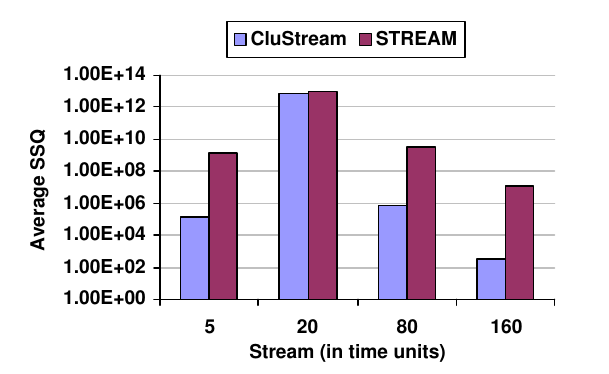
\includegraphics[width=0.9\columnwidth]{./styles/2000h1-orig.png}
%             \caption{SSQ for the original $CluStream$~\cite{clustreamOrig} vs STREAM~\cite{}}\label{fig:2000orig}
%         \end{minipage}
%         \hfill{}
%         \begin{minipage}[r]{1.0\columnwidth}
%             \centering
%             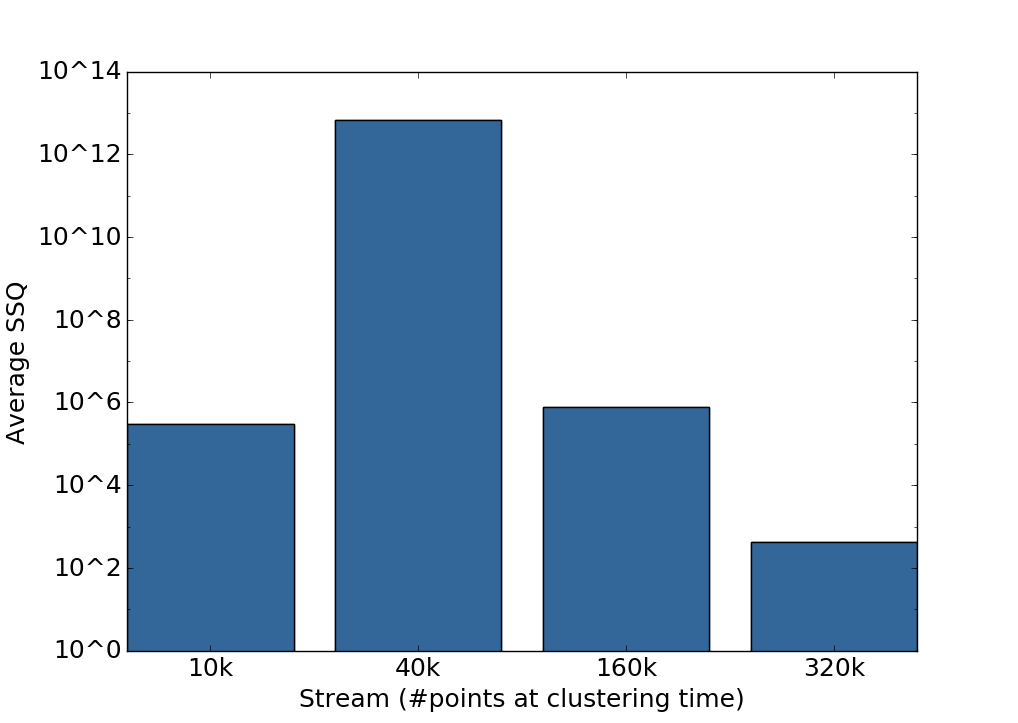
\includegraphics[width=0.9\columnwidth]{./styles/2000h1.png}
%             \caption{SSQ for our $Spark-CluStream$}\label{fig:2000}
%         \end{minipage}
%         \captionsetup{labelformat=empty}
%         \caption{Original $CluStream$ vs SPARK-Clustream.  $DS1$ (Stream speed $v$ = 2,000, $H$=1).}
%         \label{fig:DS1quality}
%     \end{figure*}
    
% Figure \ref{fig:2000orig} shows the results used by the original \textit{CluStream} to show its capabilities against an older method \textit{STREAM}, which is a modified version of K-Means for data streams. The average SSQ for \textit{CluStream} is the most relevant to this test.

% \addtocounter{figure}{-1}
% 
\paragraph{Results for DS2}
% <<<<<<< HEAD
% The SSQ for $DS2$ is shown in Figure~\ref{fig:DS2quality}.
%     \begin{figure*}[!ht]
% =======
% The SSQ for $DS2$ is shown in Figure \ref{fig:DS2quality}.
%  \begin{figure*}[!ht]
>>>>>>> b48fee025a90694a4c09982cc46b20463adc1770
%         \begin{minipage}[l]{1.0\columnwidth}
%             \centering
%              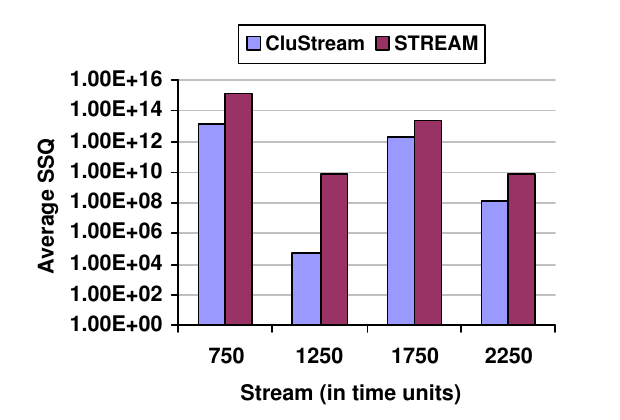
\includegraphics[width=0.9\columnwidth]{./styles/200h256-orig.png}
%             \caption{SSQ for the original $CluStream$~\cite{clustreamOrig} vs STREAM~\cite{}}\label{fig:200h256-orig}
%         \end{minipage}
%         \hfill{}
%         \begin{minipage}[r]{1.0\columnwidth}
%             \centering
%             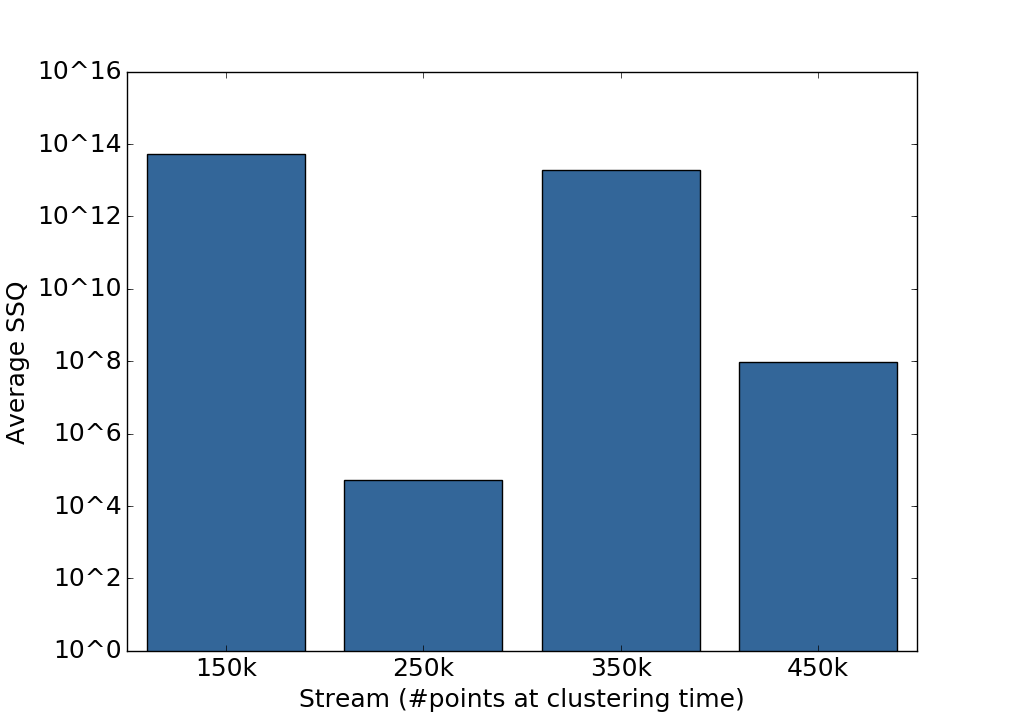
\includegraphics[width=0.9\columnwidth]{./styles/200h256.png}
%             \caption{SSQ for our $Spark-CluStream$}\label{fig:200h256}
%         \end{minipage}
%         \captionsetup{labelformat=empty}
%         \caption{Original $CluStream$ vs SPARK-Clustream. $DS2$ (Stream speed $v$ = 200, $H$=256).}
%         \label{fig:DS2quality}
%     \end{figure*}
% <<<<<<< HEAD
% =======
%     
%  \addtocounter{figure}{-1}
%  
 
% >>>>>>> b48fee025a90694a4c09982cc46b20463adc1770
Parameters were set as for $DS1$.
% The measurement is the SSQ again and the same circumstances apply for this case as in the first one with the difference that here $\delta$ and $m$ are relevant. The parameter $m$ is again chosen to be 20: if 200 points are processed every time unit and there are 50 micro-clusters, assuming all 200 points should be distributed uniformly at least every 5 time units leads to $5\frac{200}{50}=20$. An in-depth analysis of the behavior of \textit{CluStream} for different $\delta$'s and $m$'s is out of the scope of this work. 
% Again, the comparison is for the average SSQ. 
% <<<<<<< HEAD
% The test ran 4 times for \textit{Spark-CluStream} to average the results in both cases, $DS1$ and $DS2$. \color{red} Same for DS1? You run the streams x4 and reported the avg values over the 4 runs?\color{black}\color{blue}Yes, the same process was used\color{black}
The exact scores of \our~and the approximate values from \clustream~are reported %shown in Figure~\ref{fig:DS2quality}; again, they perform similarly. The exact SSQ scores for $Spark-CluStream$ and the approximated ones from $CluStream$ based on~\cite{CluStream} are shown 
in Table~\ref{tab:DS2quality}. Again the quality scores are comparable, i.e., our \our~achieves similar quality clusterings to the original \clustream.
% =======
% The test ran 4 times for \textit{Spark-CluStream} to average the results in both cases, $DS1$ and $DS2$. 
% Again, they perform similarly. The exact SSQ scores for $Spark-CluStream$ and the approximated ones from $CluStream$ based on \cite{clustreamOrig} are shown in Table \ref{tab:DS2quality}.

% >>>>>>> b48fee025a90694a4c09982cc46b20463adc1770
\begin{table*}[t]
\centering
\begin{tabular}{|l|l|l|l|l|}\hline
\textbf{$DS2$ - avg SSQ} & \textbf{150k} & \textbf{250k} & \textbf{350k} & \textbf{450k}\\\hline
CluStream & $10^{13}$-$10^{14}$ & $\approx 10^{5}$ & $10^{12}$-$10^{13}$ & $\approx 10^{8}$\\\hline
Spark-CluStream & $5.402\times10^{13}$ & $5.143\times10^{4}$ & $1.892\times10^{13}$ & $9.646\times10^7$\\\hline
  \end{tabular}
  \caption{$DS2$ - Average SSQ values}
  \label{tab:DS2quality}
\end{table*}

%------------------------------------------------------------------------------------------------------
\subsubsection{$Spark-CluStream$ vs other clustering approaches in SPARK}
\label{sec:expQuality-vs-SPARK}
% <<<<<<< HEAD
We compare our \our against available solutions for stream clustering in Spark and in particular against\textit{Streaming K-Means}~\footnote{More information: https://databricks.com/blog/2015/01/28/introducing-streaming-k-means-in-spark-1-2.html} and\textit{StreamDM-CluStream}~\footnote{More information: http://huawei-noah.github.io/streamDM/}.
% =======
% We compare our \our  against available solutions for stream clustering in Spark and in particular against \textit{Streaming K-Means} and \textit{StreamDM-CluStream}.
% >>>>>>> b48fee025a90694a4c09982cc46b20463adc1770
% , which is another adaptation of \textit{CluStream} for Spark. 
We report here on their clustering quality, the efficiency issue is discussed in Section~\ref{sec:expScalability}.

% We roughly overview these methods hereafter.

% The setup and the dataset are the same as in \ref{validation}, as having already verified results provides the possibility of using those tests to directly compare the results against the other methods. Again, the used measurement is the sum of squares (SSQ).

% Before looking at the results, here are some key considerations for the other methods:

% <<<<<<< HEAD
% \begin{itemize}%  \item \textit{Streaming K-Means~\footnote{More information: https://databricks.com/blog/2015/01/28/introducing-streaming-k-means-in-spark-1-2.html}}:
%  \begin{itemize}
%   \item In order to have comparable results, the time horizon $H$ must be interpreted differently. There are two strategies: the first option is to use the parameter \textit{halfLife}, which can be configured to let the algorithm to completely adjust the clusters after $HL$ points or batches.
%   \item The alternative would be to set the $decayFactor$, which sets the weight for the clusters of the "old" data (only the current batch is considered "new" data). This is a number between 0 and 1, such that if it is 0 then only the clusters for "new" data determine the final clusters, if it is set to 1, then the clusters of past data will have the same influence on the final clusters. It is important to notice that this \textit{decayFactor} also considers the number of points of the "new" and "old" data, so in the last case, after a long time, "new" data will have little influence as the number of points of the current batch will be considerable smaller than the points clustered so far.
%  \end{itemize}
%  \item \textit{StreamDM-CluStream~\footnote{More information: http://huawei-noah.github.io/streamDM/}}:
%  \begin{itemize}
%   \item This adaptation of \textit{CluStream} does not include the offline part as a separate module, meaning that it does not save snapshots and therefore it has to perform the macro-clustering process for every batch. This brings some limitations, the horizon $H$ no longer has the same meaning: the $\delta$ parameter is used instead as an equivalent, relying on the micro-clustering part only and its ability to delete and create new micro-clusters.
% \end{itemize}
% \end{itemize}
% \color{black}
% =======
% \begin{itemize}
%  \item \textit{Streaming K-Means~\footnote{More information: https://databricks.com/blog/2015/01/28/introducing-streaming-k-means-in-spark-1-2.html}}:
%  \begin{itemize}
%   \item In order to have comparable results, the time horizon $H$ must be interpreted differently. There are two strategies: the first option is to use the parameter \textit{halfLife}, which can be configured to let the algorithm to completely adjust the clusters after $HL$ points or batches.
%   \item The alternative would be to set the $decayFactor$, which sets the weight for the clusters of the "old" data (only the current batch is considered "new" data) to calculate the new centroids.
%  \end{itemize}
%  \item \textit{StreamDM-CluStream~\footnote{More information: http://huawei-noah.github.io/streamDM/}}:
%  \begin{itemize}
%   \item This adaptation of \textit{CluStream} does not include the offline part as a separate module, meaning that it does not save snapshots and therefore it has to perform the macro-clustering process for every batch. This brings some limitations, the horizon $H$ no longer has the same meaning: the $\delta$ parameter is used instead as an equivalent, relying on the micro-clustering part only and its ability to delete and create new micro-clusters.
% \end{itemize}
% \end{itemize}
% >>>>>>> b48fee025a90694a4c09982cc46b20463adc1770

\paragraph{Results on $DS1$}
For the $DS1$ stream the results are shown in Figure~\ref{fig:comparison2000}. %The number of clusters $k$ is always 5 for this dataset in all the experiments.
For \textit{Streaming K-Means}, the horizon $H=1$ is transformed to $halfLife=1,000$ points, as the stream speed is 2,000 points. %This is because the speed of the stream is 2,000 points per time unit, if the horizon is 1, then only 2000 points are desired to be clustered, and half of that results in 1000 points. 
The \textit{decayFactor} is set to 0, i.e., only the last 2,000 points will influence on the clusters. %, which is exactly what is desired.
\textit{StreamDM-CluStream} is set up with its default parameters, only changing the horizon to 1 and the number of micro-clusters to 50 to match those of \our.
%
\begin{figure}[h]
 \centering
 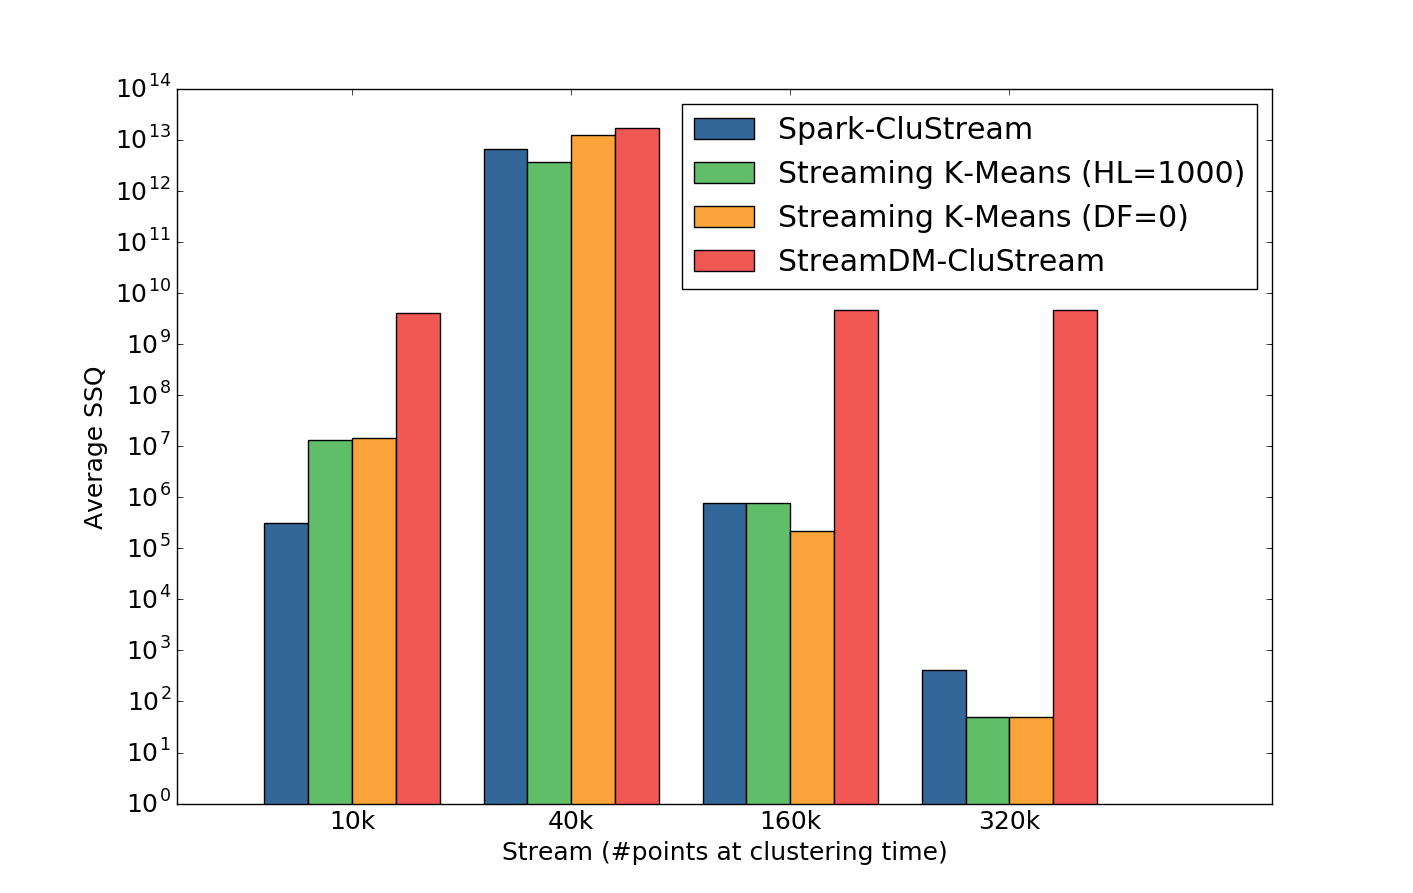
\includegraphics[scale=0.265]{./styles/comparison2000.png}
 \caption{Average SSQ for different stream clustering methods in SPARK. $DS1$ (Stream speed $v$ = 2,000, $H$=1)}
 \label{fig:comparison2000}
\end{figure}
% <<<<<<< HEAD
%
As we can see, our \our~delivers results which are very close to those of \textit{Streaming K-Means}, whereas \textit{Streaming K-Means} with the \textit{decayFactor} (DF) is the best.
% expected to do well on this test as it could be configured to cluster exactly as it was intended for this dataset. 
The surprising results come from \textit{StreamDM-CluStream}, which is the worse among the tested methods, especially for the last two points, i.e., at $160k$ and $320k$.
% To understand this behavior, we performed another experiment with \our~without snapshots. For both methods we used a horizon $H = 1$ and $m=100$. 
% \color{red}@Omar: what is m?\color{black}\color{blue}UPDATED THE EXPLANATION ABOVE \color{black}.
To further investigate this, we conduct another experiment where we compare \our~without snapshots against \textit{StreamDM-CluStream}. The results are shown in Figure \ref{fig:comparisonNoSnaps}.
% =======

% From Figure~\ref{fig:comparison2000} it can be seen that our \our~delivers results which are very close to those of \textit{Streaming K-Means}. Also, \textit{Streaming K-Means} with the \textit{decayFactor} (DF) is expected to do well on this test as it could be configured to cluster exactly as it was intended for this dataset. 
% The surprising results come from \textit{StreamDM-CluStream}, as it performs worse than the rest of the methods, especially for the last two points, i.e.,  at $160k$ and $320k$.
% To understand this behavior, we performed another experiment with \our~without snapshots. For both methods we used a horizon $H = 1$ and $m=100$.
% >>>>>>> b48fee025a90694a4c09982cc46b20463adc1770
\begin{figure}[h]
 \centering
 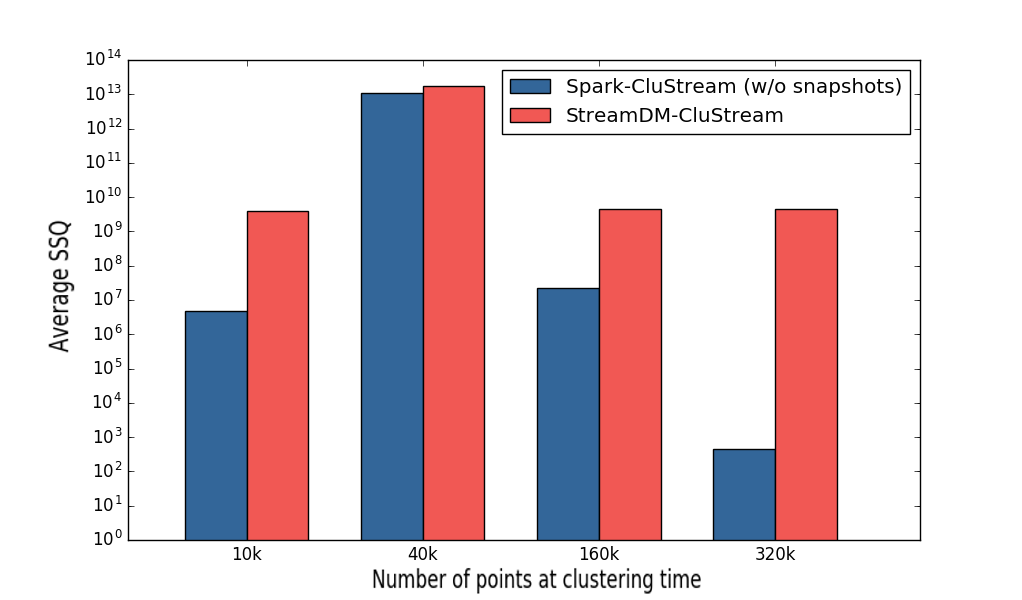
\includegraphics[scale=0.24]{./styles/comparisonNoSnaps.png}
 \caption{\our without snapshots vs \textit{StreamDM-CluStream}. $DS1$ (Stream speed $v=2,000$, $H=1$, $m=100$).}
 \label{fig:comparisonNoSnaps}
\end{figure}
As we can see, \our outperforms \textit{StreamDM-CluStream} even if we remove the snapshot part, but the quality is lower comparing to the snapshot version.
%  shows poorer results for \textit{Spark-CluStream} in comparison to its original behavior with snapshots, but still delivers noticeably better results than \textit{StreamDM-CluStream}, even though all these tests were executed 4 times and the SSQ erros were averaged to get a better representation of how these methods perform.

%-------------------------------------
\paragraph{Results on $DS2$}
% <<<<<<< HEAD
For the $DS2$ stream the results are shown in Figure~\ref{fig:comparison200}.
% Repeating the experiment for the stream with a speed of 200 and a horizon $H=256$ revealed unexpected results. 
All parameters remained the same for all methods, except for the $halfLife$ parameter for \textit{Streaming K-Means}, which is set to  $halfLife=25,600$ ($200\cdot 256=51,200$).
% We computer the new $halfLife$ as follows: multiplying the speed of the stream to the horizon, $200\cdot 256=51200$ shows how many points of the stream are supposed to be clustered at each time, indicating that the parameter should be set to $halfLife=25,600$. 
We calculate the $decayFactor$ as follows: 
% The \textit{decayFactor} strategy at first seems that does not work for such an experiment, but considering that the total number of entries and the exact clustering points are known, it is possible to calculate an average value to use as a $decayFactor$:  
% \begin{itemize}
%  \item 
At 150,000 points, the ratio of the points to cluster to the total number of points at that particular time is $\frac{51,200}{150,000} \approx 0.3413$.
%  \item 
At 250,000 points, this equals to $\frac{51,200}{250,000} \approx 0.2048$.
%  \item 
At 350,000 points, this equals to $\frac{51,200}{350,000} \approx 0.1462$.
%  \item 
At 450,000 points, this equals to $\frac{51,200}{450,000} \approx 0.1137$.
% \end{itemize}
Averaging those ratios leads to a \textit{decayFactor = 0.2015}. %, which is a way to determine how important the old data is in comparison to the new one.
\begin{figure}[h!]
 \centering
 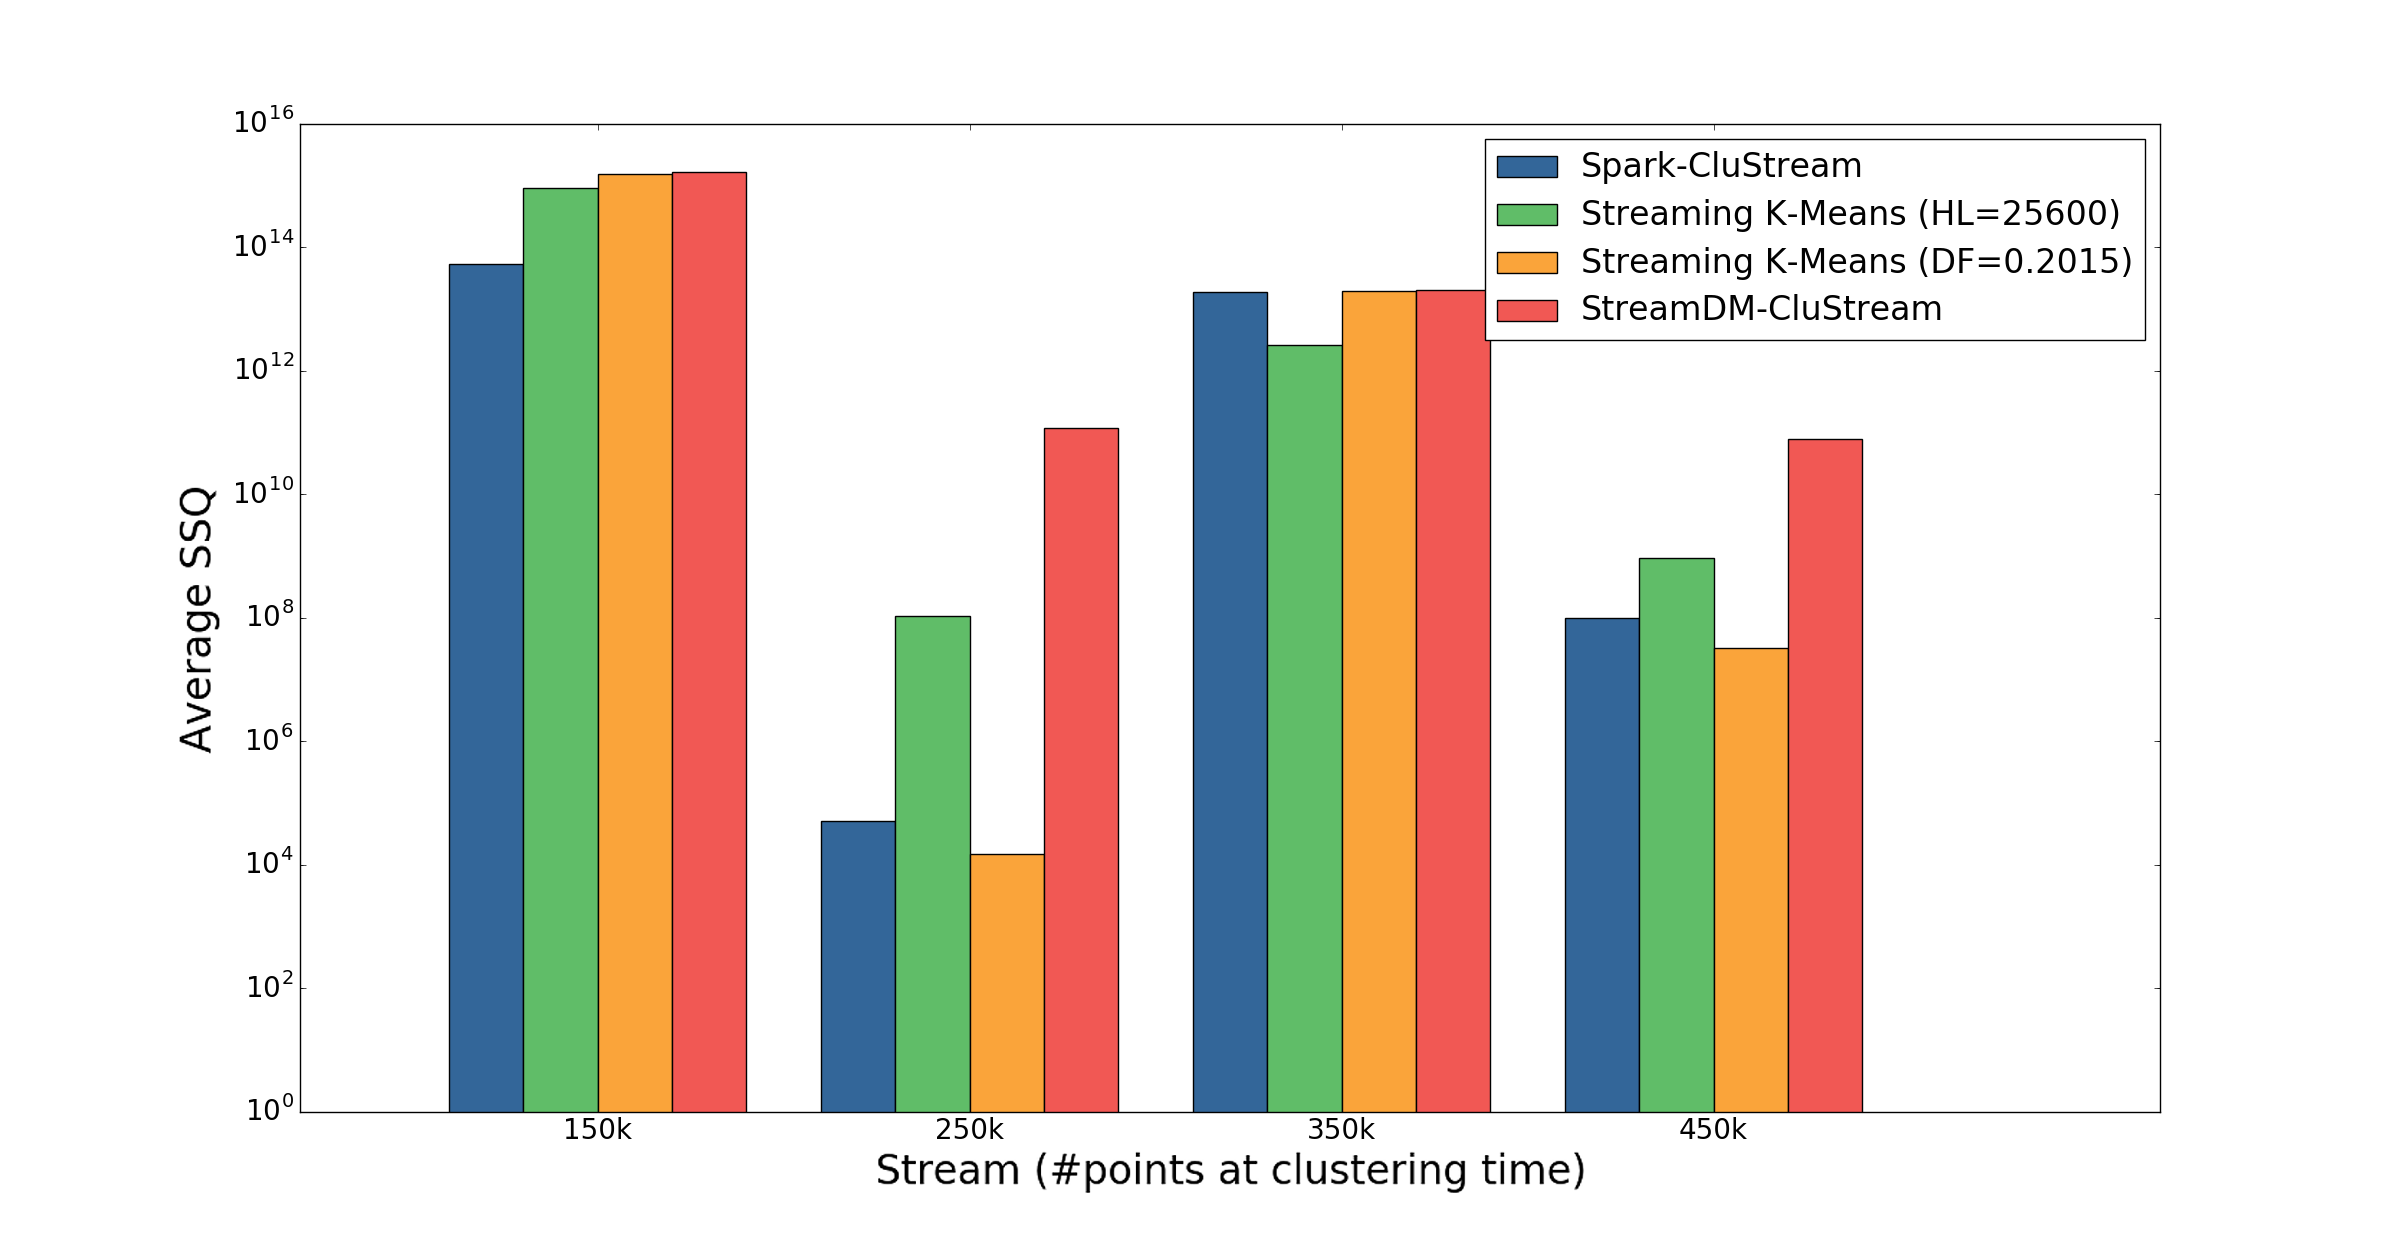
\includegraphics[scale=0.15]{./styles/comparison200.png}
%  \caption{Comparison results: all methods. Stream speed = 200, H=256}
 \caption{Average SSQ for different stream clustering methods in SPARK. $DS2$ (Stream speed $v$ = 200, $H$=256)}
 \label{fig:comparison200}
\end{figure}
As we can see, \our performs consistently well and better than \textit{StreamDM-CluStream}. As expected \textit{Streaming K-Means} with the \textit{decayFactor} achieves the best performance.

We repeat the without-snapshot experiment, the results are shown in Figure \ref{fig:comparisonNoSnaps2}.
\begin{figure}[h]
 \centering
 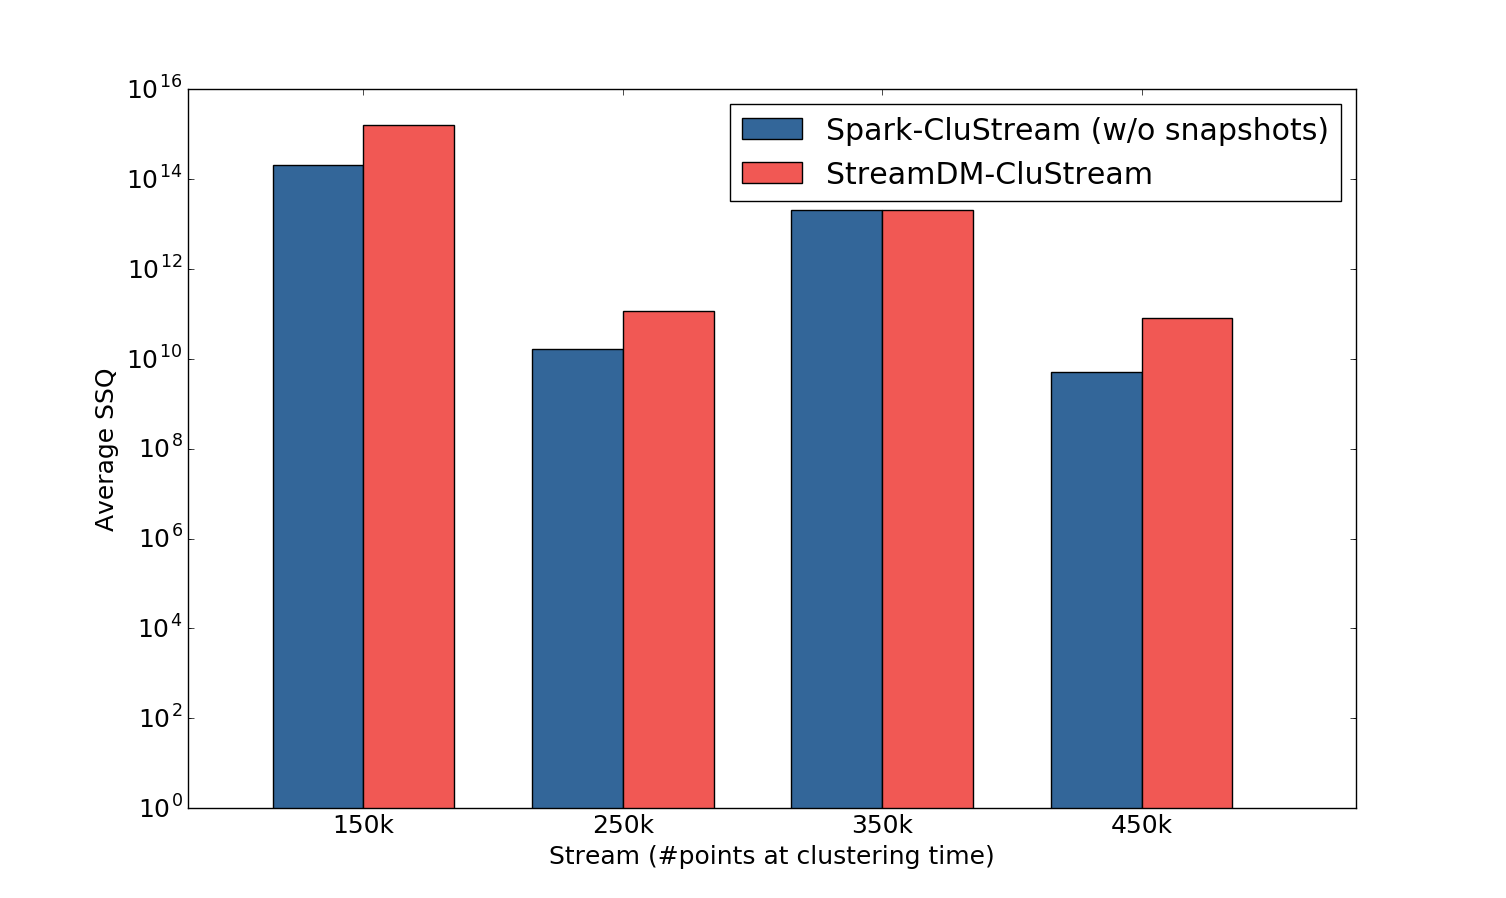
\includegraphics[scale=0.24]{./styles/comparisonNoSnaps2.png}
  \caption{\our without snapshots vs \textit{StreamDM-CluStream}. $DS2$ (Stream speed $v=200$, $H=256$, $m=100$).}
 \label{fig:comparisonNoSnaps2}
\end{figure}
As we can see, \our~delivers better results than \textit{StreamDM-CluStream} but the difference is reduced significantly comparing to $DS1$. These results might indicate that \textit{StreamDM-CluStream}  benefits from larger horizons.
% =======
% For the $DS2$ stream the results are shown in Figure~\ref{fig:comparison2000}.

% Repeating the experiment for the stream with a speed of 200 and a horizon $H=256$ revealed unexpected results. While most parameters for all methods remained the same, for \textit{Streaming K-Means} a new $halfLife$ has to be calculated: multiplying the speed of the stream to the horizon, $200\cdot 256=51200$ shows how many points of the stream are supposed to be clustered at each time, indicating that the parameter should be set to $halfLife=25600$. 


% The \textit{decayFactor} strategy at first seems that does not work for such experiment, but considering that the total number of entries is known and exactly the marks at which the clustering process happens, it is possible to calculate an average value to use as a $decayFactor$: 

% \begin{itemize}
%  \item At 150000 points: $\frac{51200}{150000} \approx 0.3413$, which is the ratio of the points to cluster to the total number of points at that particular time.
%  \item At 150000 points: $\frac{51200}{250000} \approx 0.2048$.
%  \item At 150000 points: $\frac{51200}{350000} \approx 0.1462$.
%  \item At 150000 points: $\frac{51200}{450000} \approx 0.1137$.
% \end{itemize}

% Averaging those ratios leads to a \textit{decayFactor = 0.2015}, which is a way to determine how important the old data is in comparison to the new one.

% \begin{figure}[h!]
%  \centering
%  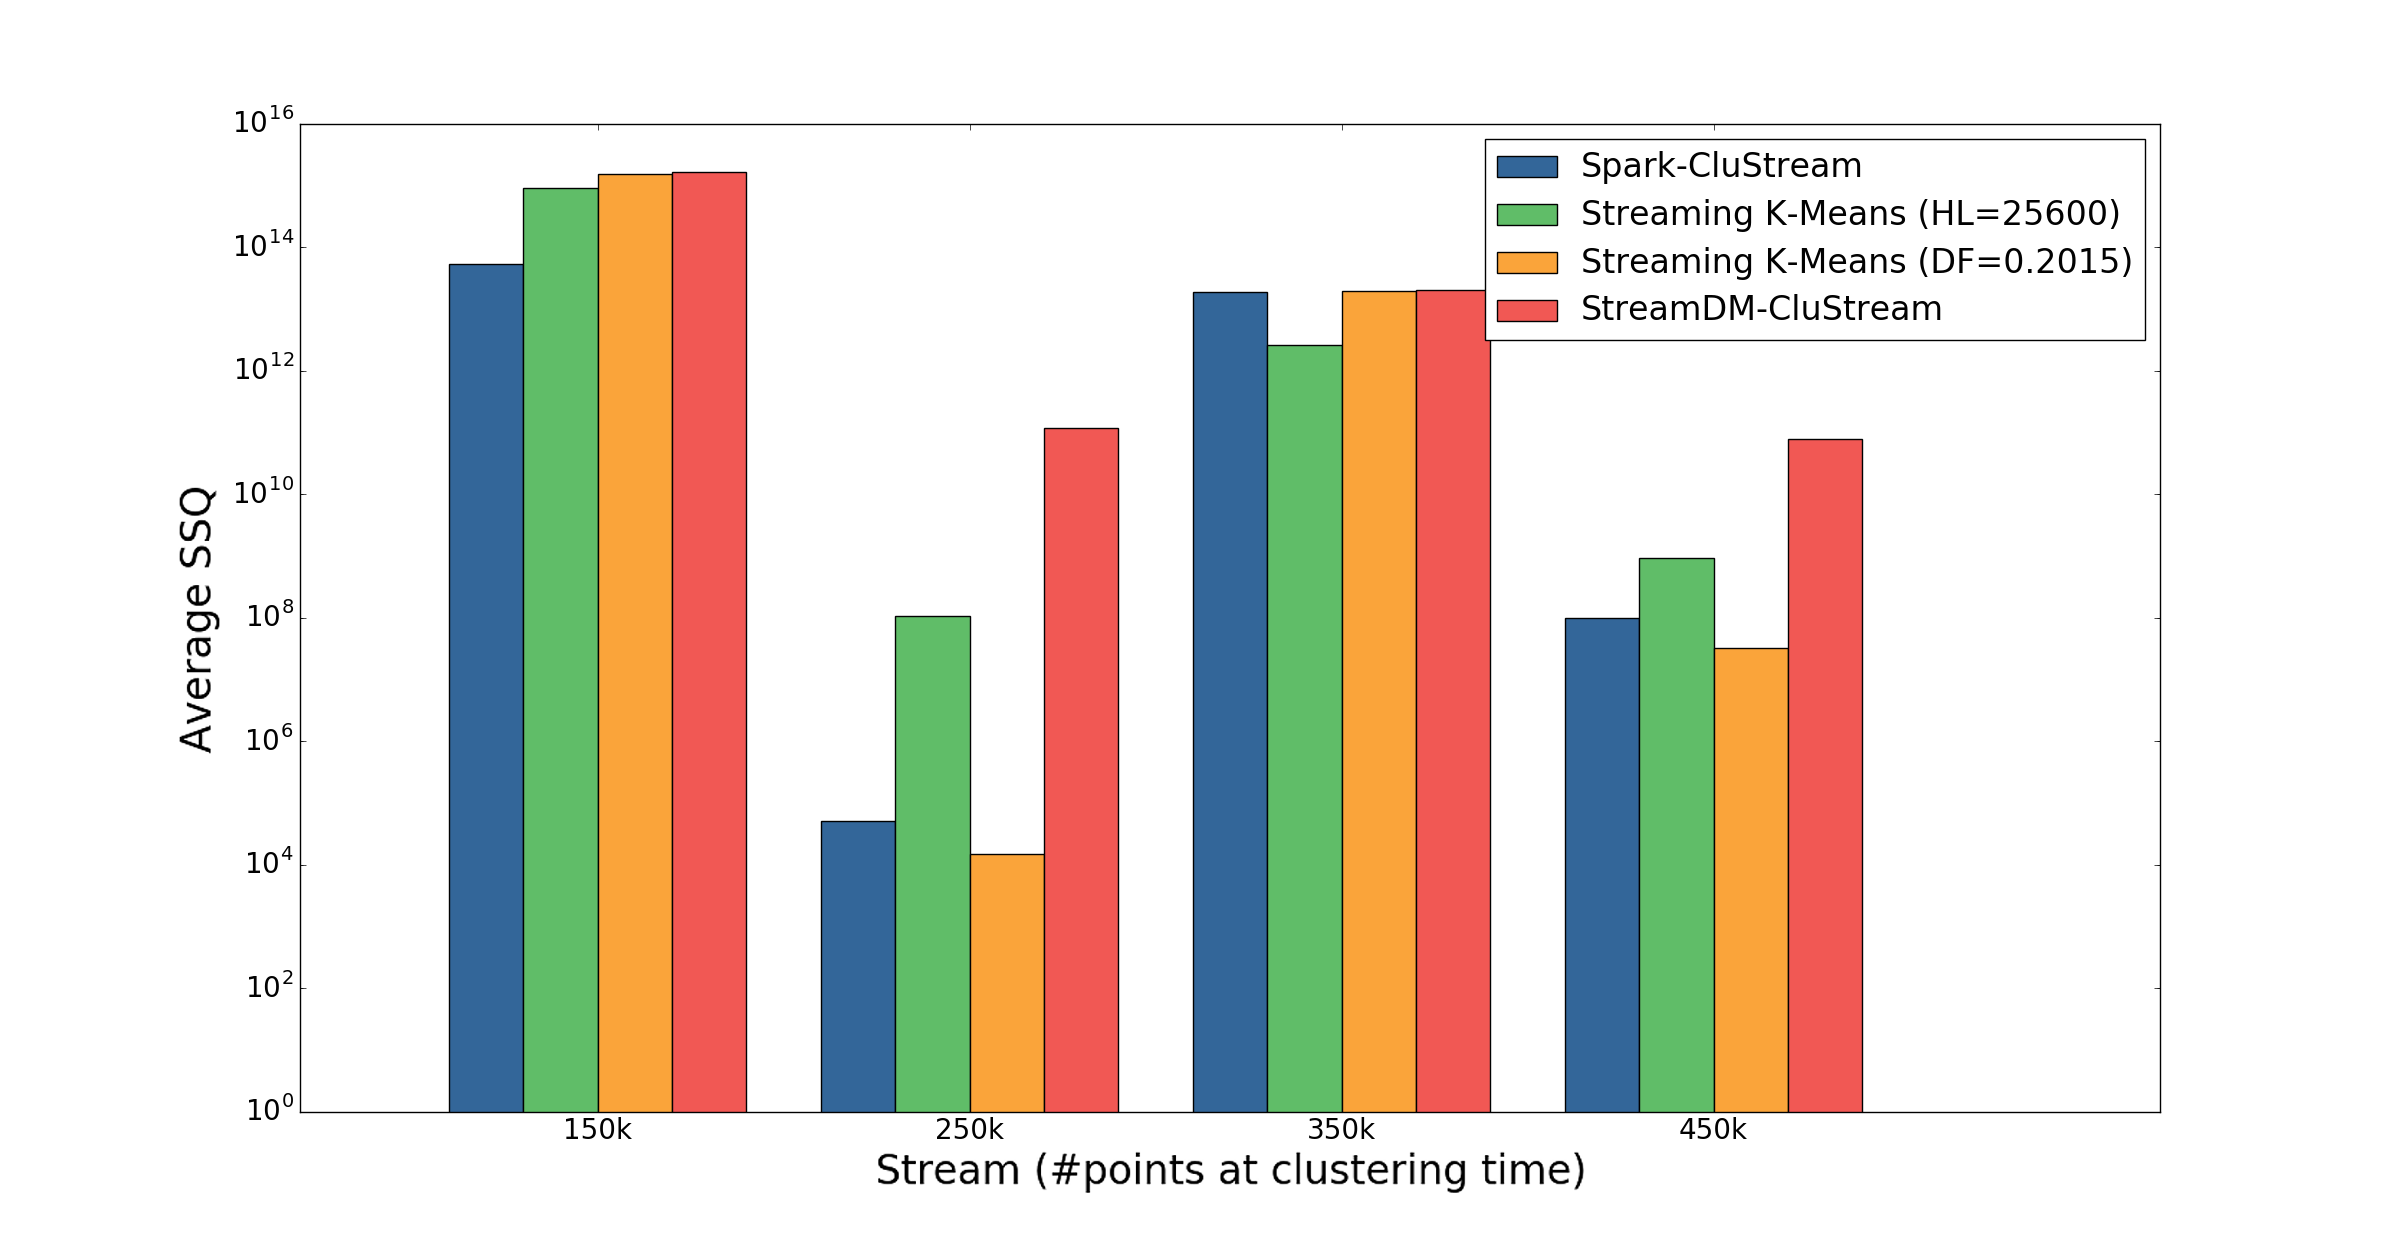
\includegraphics[scale=0.16]{./styles/comparison200.png}
%  \caption{Comparison results: all methods. Stream speed = 200, H=256}
%  \label{fig:comparison200}
% \end{figure}

% Figure \ref{fig:comparison200} shows that while \textit{Spark-CluStream} still performs consistently good, \textit{Streaming K-Means} with the \textit{decayFactor} outperformed its relative with the $halfLife$ strategy. Another thing to notice is that \textit{StreamDM-CluStream} still delivered the worse results. 


% >>>>>>> b48fee025a90694a4c09982cc46b20463adc1770



%------------------------------------------------------------------------------------------------------
\subsection{Scalability}
\label{sec:expScalability}
We test the scalability with respect to data dimensionality and number of microclusters, using data generated by a \textit{Random Radial Basis Function} generator.

The scalability tests are performed in two different scenarios: one being an analysis of how it scales for different number of attributes (dimensions of the data points) using only 20 micro-clusters and the other one using 200 micro-clusters. The reason behind this is that the number of attributes and the number of final clusters for a specific purpose are two key factors which determine the complexity of \textit{Spark-CluStream}. The speed of the stream is controlled for 10000 points for every batch of data because it is easier to test the scalability when many computations have to be done.

Any application using Spark streaming assigns one core exclusively to handle the stream, therefore the minimum number of processors required is two, this also means that using 2 processors is equivalent to using a single processor to execute the application. The number of processors mentioned in these tests is the total, but the real number of processors used for the computations is that number minus one.


\begin{figure*}[!ht]
        \begin{minipage}[l]{1.0\columnwidth}
            \centering
             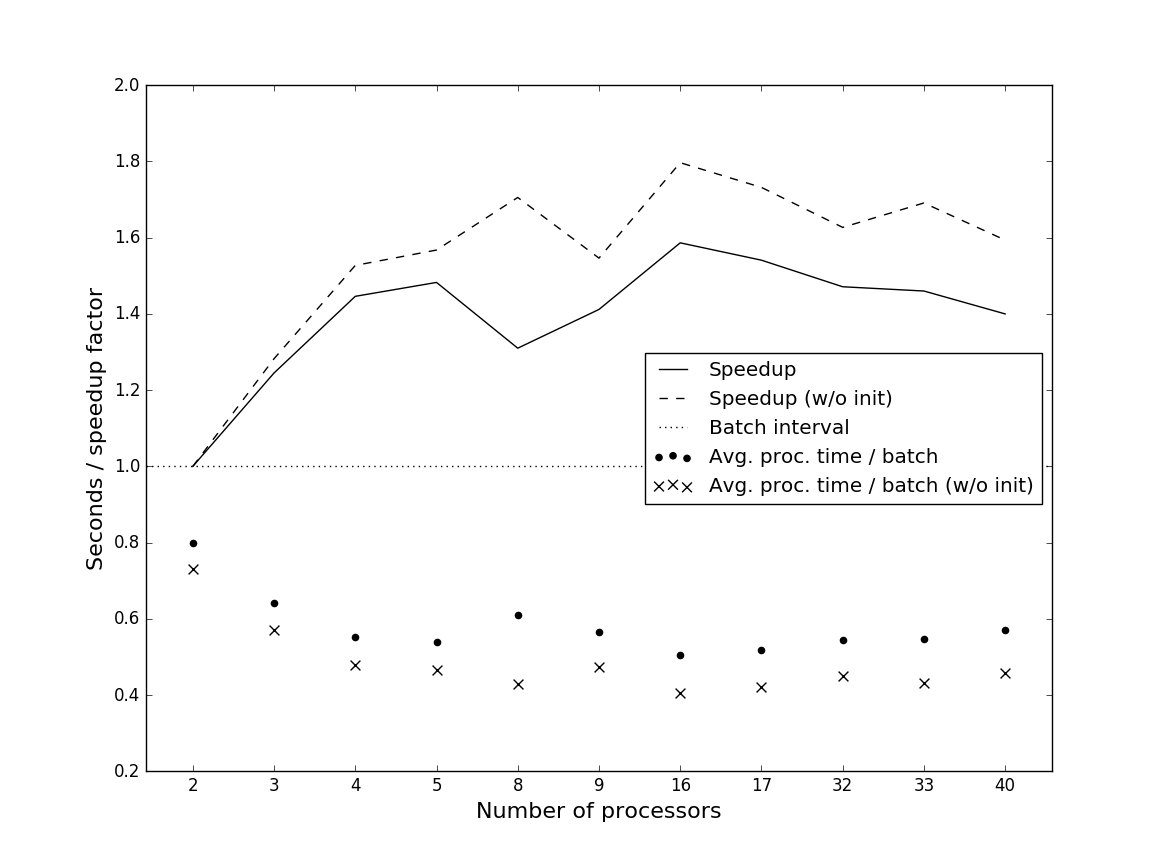
\includegraphics[width=0.9\columnwidth]{./styles/perf20-2.png}
            \caption{Dimension: $d$ = 2}
            \label{fig:perf20-2}
        \end{minipage}
        \hfill{}
        \begin{minipage}[r]{1.0\columnwidth}
            \centering
            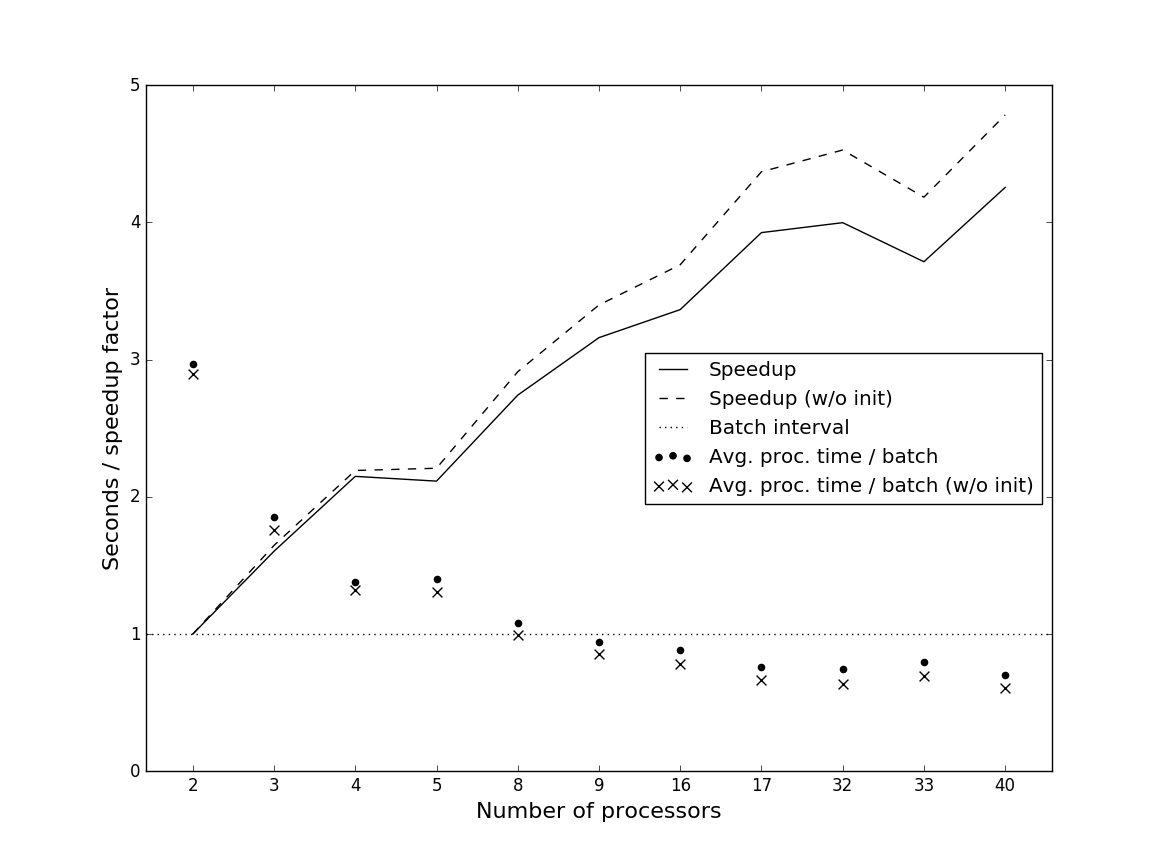
\includegraphics[width=0.9\columnwidth]{./styles/perf20-100.png}
            \caption{Dimension: $d$ = 100}\label{fig:perf20-100}
        \end{minipage}
        \captionsetup{labelformat=empty}
	\caption{Scalability-dimensionality comparison for Stream speed = 10000 and q = 20}
	 \label{fig:DS1quality}
\end{figure*}
\addtocounter{figure}{-1}
The charts here presented show the speedup obtained by increasing the number of processors from 2 to 40, which in reality means that 1 to 39 processors where used for the computations. It also shows the average processing time for each batch of data. Because the initialization takes the most amount of time, it is also convenient to show these values without considering that process: by doing so it is possible to see what would be the expected results for a longer run, where the initialization is no longer dominant. Finally it shows the interval time for which Spark process a new batch of data, in particular all these tests processed batch every second.


Figure \ref{fig:perf20-2} shows that using only 20 micro-clusters and 2 dimensions has poor scalability, not even being able to perform twice as fast as for a single processor (2 in total). Even for this high speed streaming, one processor is enough to process the batches of data before a new batch is processed, meaning that the setup is stable.

\begin{figure*}[!ht]
        \begin{minipage}[l]{1.0\columnwidth}
            \centering
             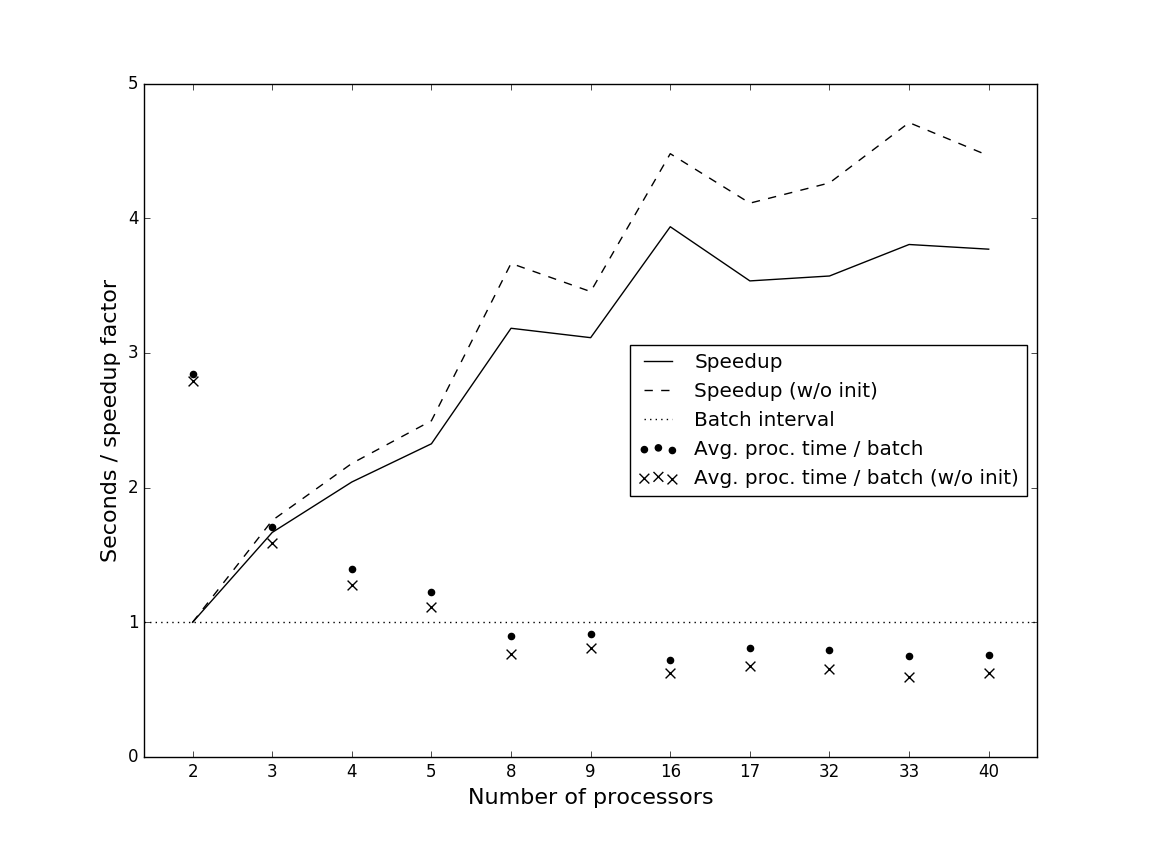
\includegraphics[width=0.9\columnwidth]{./styles/perf200-2.png}
            \caption{Dimension: $d$ = 2}
            \label{fig:perf200-2}
        \end{minipage}
        \hfill{}
        \begin{minipage}[r]{1.0\columnwidth}
            \centering
            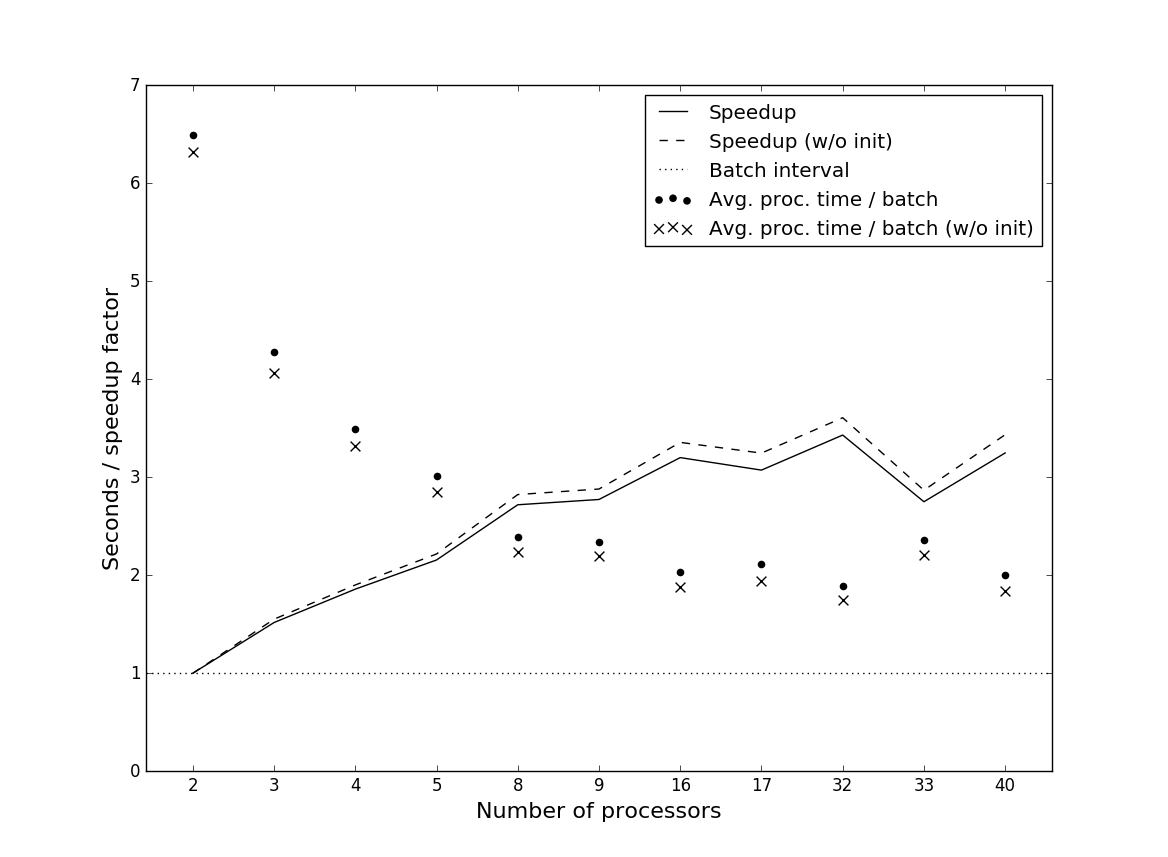
\includegraphics[width=0.9\columnwidth]{./styles/perf200-100.png}
            \caption{Dimension: $d$ = 100}\label{fig:perf200-100}
        \end{minipage}
        \captionsetup{labelformat=empty}     
        \caption{Scalability-dimensionality comparison for Stream speed = 10000 and q = 200}
        \label{fig:DS2quality}
\end{figure*}

\addtocounter{figure}{-1}
Increasing the dimensionality of the points increases the computational effort needed to process the points in every batch of data and here is where \textit{Spark-CluStream} shows its scalability, which is almost linear\footnote{By linear scalability does not mean it scales with a 1 to 1 ratio, but rather linearly proportional.} for up to 16-17 processors, as it can be seen in Figure \ref{fig:perf20-100}.  From the average processing time per batch, it can be seen that from 32 to 40 processors it does not improve much anymore and the speedup does not increase quasi-linearly anymore. Here a total of 9 processors were required to stabilize \textit{Spark-CluStream}. 


Interestingly, increasing the number of micro-clusters by a factor of 10 for 2 attributes resulted in good scalability, similarly to the scenario with 20 micro-clusters and 100 attributes. Here a total of 8 processors were enough for a stable run, as shown in Figure \ref{fig:perf200-2}.



Finally, when the number of clusters and the number of attributes are both increased significantly, Figure \ref{fig:perf200-100} shows for \textit{Spark-CluStream} quasi-linear scalability but this time only up to about 8-9 processors. After that point, the speedup slows down showing almost no improvement after 16 processors. This test never reached a stable configuration.


\subsection{Performance}

In this section, the scalability of \textit{Spark-CluStream} is compared to that of \textit{StreamDM-CluStream} and Spark's \textit{Streaming K-Means} unsing the Spark cluster setup for $q=20$ and $d=2,100$, for the $CluStream$ method. Also, a test on a signle machine is performed.


\begin{figure}[h!]
 \centering
 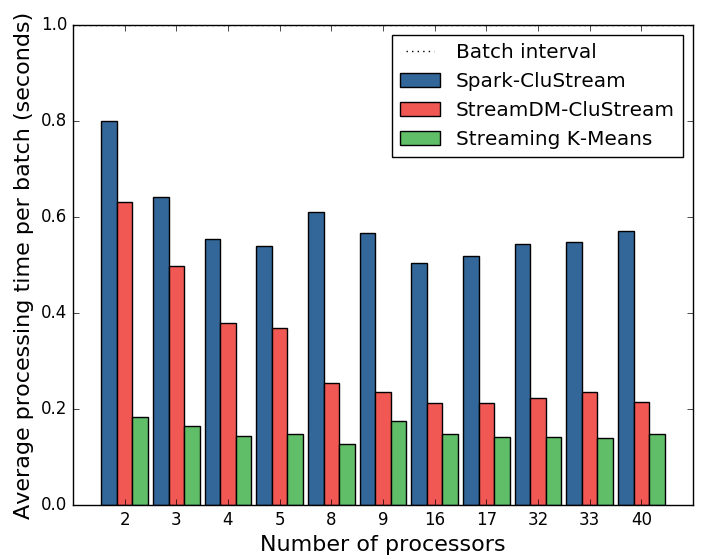
\includegraphics[scale=0.45]{./styles/perfComp2.png}
 \caption{Processing time comparison: $q=20$, $d=2$}
 \label{fig:perfComp2}
\end{figure}

In Figure \ref{fig:perfComp2} it can be seen that \textit{Spark-CluStream} took the most time on average to process a batch of data and being \textit{Streaming K-Means} the fastets among the three. 

\begin{figure}[h!]
 \centering
 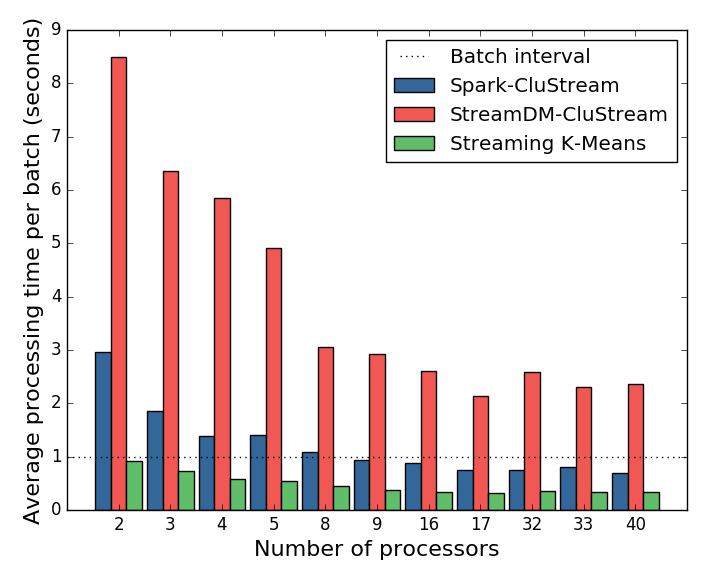
\includegraphics[scale=0.45]{./styles/perfComp100.png}
 \caption{Processing time comparison: $q=20$, $d=100$}
 \label{fig:perfComp100}
\end{figure}

When it comes to higher dimensions, \textit{Spark-CluStream} shows a significant improvement over \textit{StreamDM-CluStream}, which never got to the point were it was stable (below the 1 second mark), as shown in \ref{fig:perfComp100}, it seems to scale as fast as \textit{Spark-CluStream} but it was not enough even with 40 processors. 


\begin{figure}[h!]
 \centering
 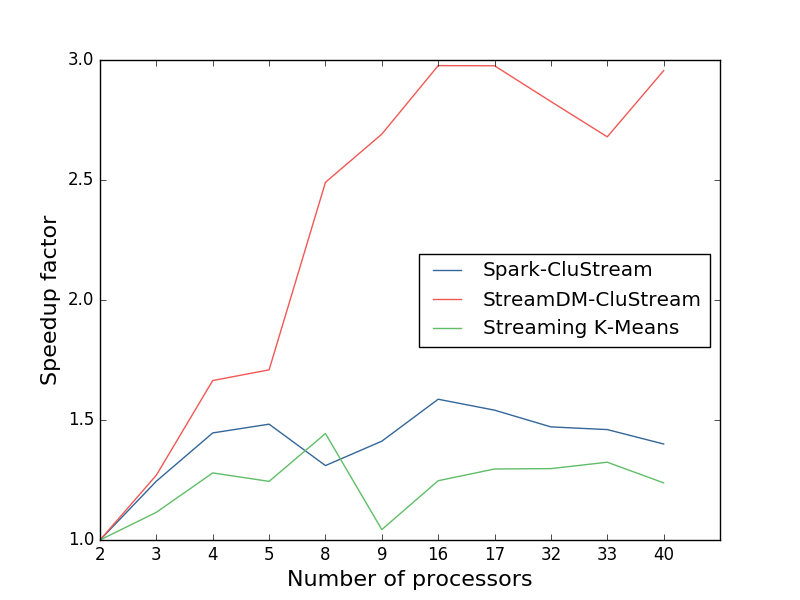
\includegraphics[scale=0.45]{./styles/scalComp2.png}
 \caption{Scalability comparison: $q=20$, $d=2$}
 \label{fig:scalComp2}
\end{figure}

Surprisingly, in Figure \ref{fig:scalComp2}, \textit{StreamDM-CluStream} shows to be able to scale even for this tests, while both \textit{Spark-CluStream} and \textit{Streaming K-Means} seem to struggle taking advantage of using more processors.

\begin{figure}[h!]
 \centering
 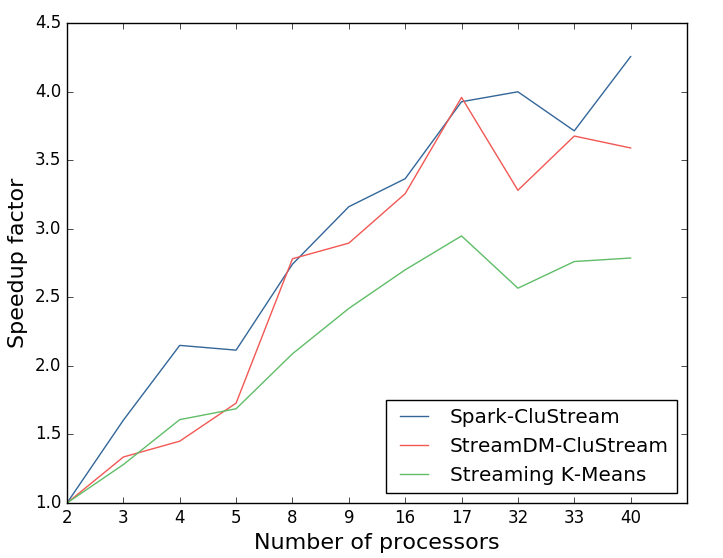
\includegraphics[scale=0.45]{./styles/scalComp100.png}
 \caption{Processing time comparison: $q=20$, $d=100$}
 \label{fig:scalComp100}
\end{figure}

Figure \ref{fig:scalComp100} shows that all three algorithms are able to scale similarly for this test, being \textit{Spark-CluStream} the one having a very slight advantage as it does not slow down as quickly as the other two.



Another interesting comparison, is the processing time per batch of data for a single machine, using a real dataset such as the \textit{Network Intrusion}. Here, communication is less of an issue as all the partitions lie in the same share memory space, and still there are 4 virtual cores in disposition for the algorithms to run. 

The test was performed using a stream speed of 2000 points per batch and with a horizon $H=1$, to match one of the validation tests.

\begin{figure}[h!]
 \centering
 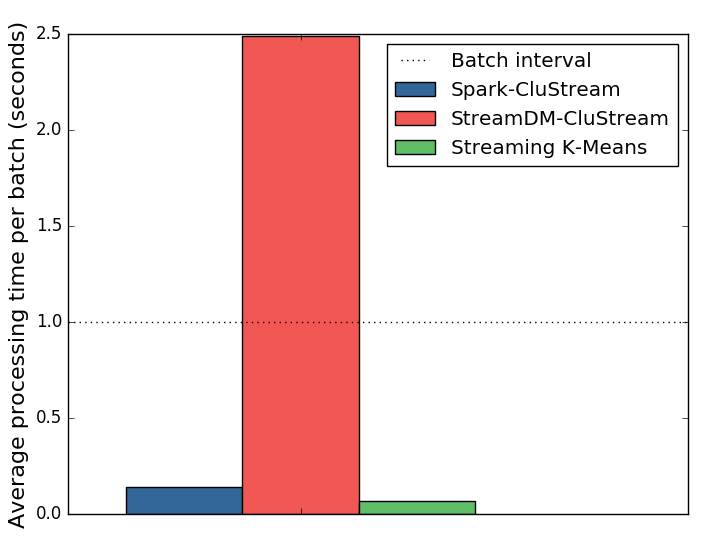
\includegraphics[scale=0.47]{./styles/singlemachine.png}
 \caption{Processing time comparison for a single machine: $q=50$, $d=34$}
 \label{fig:singlemachine}
\end{figure}

The results shown in Figure \ref{fig:singlemachine} are quite remarkable. As \textit{StreamDM-CluStream} shows a very significant disadvantage when using greater numbers of micro-clusters and higher dimensions.

For this single machine test, \textit{Spark-CluStream} was about 18 times faster on average than \textit{StreamDM-CluStream} and about two times slower than \textit{Streaming K-Means} on average.

Another consideration to be made, is that  \textit{Spark-CluStream} saves a snapshot for every batch of data, having to write to disk, while the other two algorithms never access the disk or this matter.


